\documentclass[a4paper,10pt] {article}
\usepackage{caratula}
\usepackage{a4wide}
\usepackage{graphicx}

\begin{document}

\titulo{Trabajo Pr\'actico Nro. 1}
\fecha{13/04/2009}
\materia{Algoritmos y Estructuras de Datos III}
\grupo{}
\integrante{Dinota, Mat\'ias}{076/07}{matiasgd@gmail.com}
\integrante{Huel, Federico Ariel}{329/07}{federico.huel@gmail.com}
\integrante{Leveroni, Luciano}{360/07}{lucianolev@gmail.com}
\integrante{Mosteiro, Agust\'in}{125/07}{agustinmosteiro@gmail.com}

\maketitle

\begin{center}
\section*{Ejercicio 1: La conjetura de Goldbach}
\end{center}

\bigskip
\section*{Introducci\'on}

La idea de este ejercicio es intentar demostrar de manera emp\'irica la
conjetura de Goldbach. Esta misma predica que todo n\'umero par positivo mayor
que dos se puede escribir como la suma de dos n\'umeros primos. Con este
objetivo se procedi\'o a la implementaci\'on de un algoritmo iterativo que, dado
un n\'umero par mayor que dos, retorna dos n\'umeros primos que satisfacen dicha
conjetura.

En principio, se probaron distintos casos aleatorios para encontrar un patr\'on
com\'un. A partir de esto, se realiz\'o la siguiente conjetura: ``Sea $p$ el mayor primo comprendido en el rango $3..n-2$ entonces $p$ y $n-p$ son dos n\'umeros primos cuya suma es $n$''. De ser cierta esta conjetura, bastar\'ia con hallar el primo m\'as cercano a $n-2$ para obtener, mediante operaciones ba\'asicas, el resultado esperado. Sin embargo, al poco tiempo se encontr\'o un contraejemplo ($128 = 119 + 9$, pero 9 no es primo) que falseaba la conjetura. A pesar de esto, la idea sirvi\'o para encontrar una soluci\'on al problema. En la secci\'on siguiente veremos el algoritmo en cuesti\'on.

\section*{Algoritmo}

A continuaci\'on se encuentra el pseudoc\'odigo relativo al algoritmo propuesto
que resuelve el problema, seguido de una breve explicaci\'on acerca del
funcionamiento y correctitud del mismo.

\begin{verbatim}
esPrimo(n)
  si n = 2 
    devolver true
  si n es divisible por 2
    devolver false
  para todo i par desde 3 hasta raiz de n
    si n es divisible por i
      devolver false
  devolver true

encontrarPrimos(n)
  si n = 4
    devolver (2,2)
  para todo i par desde 3 hasta n/2
    si esPrimo(i) y esPrimo(n-i)
      devolver (i,n-i)
  devolver (0,0)
\end{verbatim}

En primer lugar, se encuentr\'a la definici\'on de la funci\'on \textit{esPrimo}
que, tal como su nombre indica, retorna \textit{true} en caso de que el n\'umero
pasado como par\'amentro sea un n\'umero primo y \textit{false} en caso
contrario. El algoritmo en cuesti\'on consiste en un m\'etodo simple pero
efectivo: En primer lugar, hay 2 casos base, el primero retorna \textit{true} en caso de
tratarse del n\'umero 2 y el segundo evalua si el numero es par (divisible por
2), retornando \textit{false} en este caso, ya que todo numero par mayor que 2
no es primo. Luego, el ciclo principal evalua si el par\'ametro $n$ es divisible
por alg\'un n\'umero impar $i$ con $3 \leq i \leq \sqrt{n}$, retornando
\textit{false} en tal caso. La correctitud de tal procedimiento se desprende
directamente del teorema que predica que si $n$ es un n\'umero primo entonces
existe al menos un divisor d tal que $2 \leq d < \sqrt{n}$.

Con respecto al algoritmo relativo al problema en s\'i, la idea consiste en
recorrer todos los n\'umeros impares comprendidos entre $3$ y $n-3$ de a pares
cuya suma equivalgan a $n$. Los pares $i, n - i$ satisfacen trivialmente esta condici\'on, ya que $i + (n-i) = n$. Del mismo modo, es f\'acil ver que para generar todos los n\'umeros del rango mencionado, basta con variar i tal que $3 \le i \le n/2$. De esta forma se ve claramente que esPrimo(i) comprende el rango $3..n/2$, y $esPrimo(n-i)$ el rango $n/2..n-3$. De este modo, cuando se satisface que $esPrimo(i) \& esPrimo(n-i) == true$ se puede afirmar que se ha encontrado el par de n\'umeros que cumplen con la conjetura: dos n\'umeros primos cuya suma es $n$. En caso de que no hallar dicha tupla detro del rango propuesto, se puede concluir que la conjetura de Goldbach era falsa, retornando la tupla (0,0) en este caso.  

\section*{Complejidad}

A continuaci\'on se analizara la complejidad de peor caso sobre los modelos
uniforme y logaritmico. 

Nota: En el siguiente an\'alisis se hara referencia a funciones propias de la implementaci\'on de los algoritmos. Puede ver el c\'odigo fuente del mismo en la secci\'on \textit{Anexos}.

\subsection*{Modelo Uniforme:}

En este modelo el an\'alisis no esta centrado en el tama\~{n}o de los operandos
por lo que el tiempo de ejecuci\'on de cada operaci\'on se considera constante.

En la funci\'on esPrimo todas las operaciones y asignaciones utilizadas se
logran en tiempo constante por lo mencinado anteriormente, de esta manera la
complejidad de esta funci\'on depende del ciclo que contiene. Como itera sobre
\textit{i} entre 3 (valor de inicializaci\'on) y $\sqrt{n}+1$, y ademas en cada
vuelta del ciclo la variable es aumentada en 2, claramente se aprecia que en el
peor caso (es decir que nunca se cumpla la condici\'on n mod i = 0) el ciclo se
recorre aproximadamente $\sqrt{n}/2$ veces. De esta manera concluimos que $T(n)
\in O(\sqrt{n})$.

En cuanto a la complejidad de las operaciones y asignaciones realizadas en la
funci\'on encontrarPrimos el caso es el mismo al de esPrimo debido al modelo de
computo. La unica operaci\'on dentro del pseudocodigo de encontrarPrimos de
complejidad superior a constante es la analizada anteriormente y dicha operacion se
encuentra dentro del \'unico ciclo de la funci\'on por lo que concentraremos el
an\'alisis de complejidad aqui. En este caso iteramos sobre el mismo valor de
inicio pero el limite del ciclo esta dado por $n/2$. Tambien aqui la variable
\textit{i} es aumentada en 2 en cada iteraci\'on lo que determina que en el peor
caso se iterar\'a aproximada mente $(n/2)/2 = n/4$ veces. Como dentro del ciclo
se llama a esPrimo (complejidad $\sqrt{n}$) la complejidad final de la funci\'on
encontrarPrimos es $T(n) \in O(n*\sqrt{n})$.

\subsection*{Modelo Logar\'itmico:}

En este modelo de computo si nos concentraremos en el tama\~{n}o de la entrada y
el costo de las operaciones en funci\'on de la cantidad de bits de sus
operandos.

En la funci\'on esPrimo se puede apreciar que las operaci\'ones que mayor
complejidad conllevan son $\sqrt{n}$ y $n$ mod $i$. Como ambas son llamadas
dentro del \'unico ciclo de la funci\'on, la complejidad estar\'a determinada
por dicho ciclo.

Entonces tenemos 

$$ T(n) = \sum
[\log(\sqrt{n}+1)+\log(n)^{2}+\log(n)^{2}+\log(n\,mod\,i)+\log(i)] $$
$$\leq \sum [\log(n)+2\log(n)^{2}+\log(n)+\log(n)] $$
$$= \sqrt{n}(3\log(n)+2\log(n)^{2}) \Longrightarrow T(n) \in O(\sqrt{n}*\log(n)^{2})$$

\bigskip

Con respecto a la funci\'on encontrarPrimos sucede lo mismo con respecto a que
las operaciones de mayor complejidad son realizadas dentro del ciclo por lo que
en este caso la complejidad total de la funci\'on tambi\'en estar\'a determinada
por dicho ciclo.

La funci\'on de complejidad es 
$$ T(n) = \sum
[\log(i)+\sqrt{i}\log(i)^{2}+\sqrt{n-i}\log(n-i)^{2}+\log(n)+\log(n)+\log(i)] $$
$$ \leq \sum [\log(n)+\sqrt{n}\log(n)^{2}+\sqrt{n}\log(n)^{2}+\log(n)+\log(n)+\log(n)] $$
$$ =n(4\log(n)+2\sqrt{n}\log(n)^{2}) \Longrightarrow T(n) \in O(n^{3/2}*\log(n)^{2}) $$

\bigskip

Por \'ultimo analizaremos tambi\'en la complejidad en funci\'on del tama\~{n}o
de la entrada para los dos modelos de computo vistos. Como la funci\'on
encontrarPrimos toma unicamente un natural \textit{n}, si llamamos \textit{t} al
tama\~{n}o de entrada tenemos que $t = \log(n) \Longrightarrow 2^{t} = n$. De
esta manera, reemplazando $n$ en las complejidades calculadas previamente
obtendremos el costo de los dos algoritmos.

\begin{itemize}
\item Modelo Uniforme: 
$$T(n) \in O(n\sqrt{n}) = O(n^{3/2}) = O((2^{t})^{3/2}) =
O(2^{3t/2})$$
\item Modelo Logar\'itmico: 
$$T(n) \in O(n^{3/2}\log(n)^{2}) =
O((2^{t})^{3/2}(\log(2^{t}))^{2}) = O((2^{3t/2}t^{2})$$
\end{itemize}

\section*{An\'alisis de resultados}

Con el fin de analizar la eficiencia del algoritmo propuesto se realizaron diversas pruebas. En primer lugar, se hicieron experimentos orientados a estudiar el tiempo de ejecuci\'on del mismo en relaci\'on al par\'ametro ingresado (de ahora ne adelante, Prueba 1). Para tal prop\'osito se procedi\'o a la creaci\'on de un programa de prueba (ver pseudoc\'odigo debajo) que calcula el tiempo de ejecuci\'on de la funci\'on \textit{encontrarPrimos} para valores entre $4$ y $2^{31}-4$. Al tratarse de una cantidad de n\'umeros tan grande, como veremos m\'as adelante, la ejecuci\'on real de dicha prueba demorar\'ia en exceso (a\~{n}os). Por tal motivo se decidi\'o tomar n\'umeros pares separados por una distancia aleatoria entre $10^{4}..2*10^{4}$. La raz\'on del uso de un par\'ametro aleatorio radica en poder conseguir una buena muestra representativa del rango propuesto anteriormente y evitando as\'i casos patol\'ogicos.

\begin{verbatim}
Prueba 1
--------
mientras i <= 2^31-4
  T = tiempo que tarda la operacion encontrarPrimos(i) en microsegundos
  i = i + 10000 + numero aleatorio par entre 0 y 10000
  guardar en Ej1-Complejidad.txt la linea "i T"
\end{verbatim}

La segunda prueba tiene como objetivo mostrar que la cantidad de operaciones que realiza el algoritmo es significativa menor que la cota teorica propuestas, a\'un en los peores casos. Con este fin, se cre\'o una aplicaci\'on que obtiene los m\'aximos de la primer componente de la tupla soluci\'on (n\'umero primo mas chico) para 20 ejecuciones del algoritmo. Al igual que en la primer prueba, se opt\'o por un enfoque aleatorio, tomando muestras de n\'meros a intervalos aleatorios entre $10^{5}$ y $2*10^{5}$.

\begin{verbatim}
Prueba 2
--------
para j desde 0 hasta 20
  peor_caso_primo1 = 0
  mientras i <= 2^31-4
    <primo1, primo2> = encontrarPrimos(i)

    si primo1 > peor_caso_primo1
      peor_caso = i
      peor_caso_primo1 = primo1
      peor_caso_primo2 = primo2

    i = i + 10000 + numero aleatorio par entre 0 y 10000

  guardar en Ej1-MayoresPrimos.txt la linea "peor_caso peor_caso_primo1 peor_caso_primo2"
\end{verbatim}

Por \'ultimo, con el fin de observar m\'as en detalle el comportamiento del algoritmo se decidi\'o extraer los peores casos de la Prueba 1 y estudiarlos en profundidad (Prueba 3). Para realizar esta tarea, se implement\'o una sencilla aplicaci\'on (ver pseudoc\'odigo debajo) que tomalrededor de 200 secuencias consecutivas de 1000 n\'umeros aleatorios comprendidas entre $4$ y $2^{31}-4$ utilizando el mismo criterio que en el caso anterior. Luego, obtiene el m\'aximo tiempo de ejecuci\'on entre todos los n\'umeros de cada secuencia. 

\begin{verbatim}
Prueba 3
--------
j = 1
mientras i <= 2^31-4
  maximo_tiempo = 0
  T = tiempo que tarda la operacion encontrarPrimos(i) en microsegundos

  si T > maximo_tiempo
    maximo_tiempo = T
    peor_caso = i

  si j = 1000
    guardar en Ej1-Peorescasos.txt la linea "peor_caso maximo_tiempo"
  
  j = j + 1
  i = i + 10000 + numero aleatorio par entre 0 y 10000
\end{verbatim}

A continuaci\'on se presentan los resultados relativos a la primera aplicaci\'on (Prueba 1).

\begin{center}
 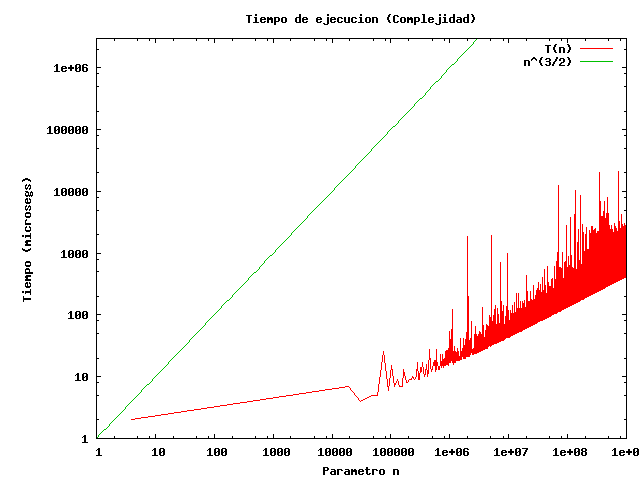
\includegraphics[width=0.7\textwidth]{Plots/Ej1-Complejidad.png}
\begin{center}
Figura 1.1
\end{center}
\end{center}

Este gr\'afico muestra la comparaci\'on entre las mediciones de tiempo de la primera prueba realizada y la complejidad te\'orica expuesta anteriormente. Llamaremos $f$ a la funci\'on que relaciona el tiempo de ejecuci\'on con el tama\~{n}o de entrada. Como se puede apreciar, el crecimiento de $f$ es mucho menor que la complejidad te\'orica, por lo cual el algoritmo resulta mucho m\'as eficiente que lo esperado. Sin embargo, a pesar de su comportamiento altamente irregular, se puede apreciar que el tiempo de ejecuci\'on aumenta a medida que crece el tama\~{n}o de la entrada. La raz\'on de la discrepancia entre ambas funciones reside un hecho que denominaremos ``el lema de la aproximaci\'on asintotica natural en el anillo conmutativo modelado implicitamente por los numeros primos y sus respectivas operaciones''. La raz\'on de la discrepancia entre ambas funciones reside en el hecho de que el algoritmo implementado encuentra dos n\'umeros primos que cumplen con la conjetura en una muy baja cantidad de operaciones en relaci\'on al taman\~{n}o de la entrada. Si bien se desconoce el motivo de este fen\'omeno, hemos probado emp\'iricamente que esto se cumple como se puede notar en el siguiente gr\'afico (Prueba 2).

GRAFICO

% \begin{center}
%  \includegraphics[width=0.7\textwidth]{Plots/Ej1-cosa.png}
% \begin{center}
% Figura 1.2
% \end{center}
% \end{center}

Como se observa en la Figura 1.2, para los peores casos la diferencia entre cada uno de los primos soluci\'on es muy alta, muy cercana al par\'ametro de entrada $n$. Esto explica que la complejidad te\'orica no se corresponda con el tiempo de ejecuci\'on.

\begin{center}
 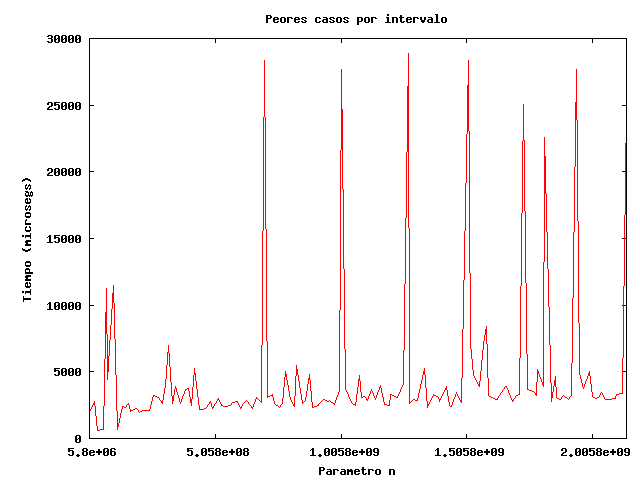
\includegraphics[width=0.7\textwidth]{Plots/Ej1-PeoresCasos.png}
\begin{center}
Figura 1.3
\end{center}
\end{center}

La idea de este gr\'afico es mostrar c\'uan irregular es el tiempo de ejecuci\'on del algoritmo. A pesar de haber hecho el esfuerzo de buscar los peores casos (mediante la aplicaci\'on de la Prueba 3), el tiempo que demoran los mismos difieren entre ellos considerablemente. Esto muestra que los peores casos no tienen una ralaci\'on directa con el tama\~{n}o de la entrada sino mas bien con la distribuci\'on desconocida de los n\'umeros primos pertenecientes al intervalo estudiado.

%TODO: explicacion de rand
%cita de casos patologicos
%mejores to do's

\section*{Conclusiones}

TODO

\begin{center}
\section*{Ejercicio 2: Resolucion de Puzzle}
\end{center}

\bigskip
\section*{Introducci\'on}

TODO

\section*{Algoritmo}

TODO

\section*{Complejidad}

TODO

\section*{An\'alisis de resultados}

TODO

\section*{Conclusiones}

TODO

\begin{center}
\section*{Ejercicio 3: C\'alculo de la mediana entre dos vectores}
\end{center}

\bigskip
\section*{Introducci\'on}

EL problema que plantea este ejercicio es calcular la mediana entre dos vectores de n\'umeros enteros, es decir, el elemento que, una vez concatenados y ordenados los vectores, deja a ambos lados la misma cantidad de elementos. Seg\'un lo especificado en el problema, ambos vectores tienen la misma longitud y est\'an ordenados.

En principio, la soluci\'on trivial del problema fue descartada ya que el costo de realizarla era excesivo para los fines del ejercicio. Esta soluci\'on consist\'ia en concatenar ambos vectores, ordenarlos y posteriormente obtener la mediana a partir del elemento medio de dicha secuencia.

Descartada esta opci\'on, surgi\'o la idea de desechar una gran cantidad de elementos, cuando sea posible, para poder realizar los c\'alculos sobre una cantidad de n\'umeros considerablemente inferior a la inicial. De esta manera, la complejidad resultar\'ia del costo de descartar los elementos apropiados y luego hacer el c\'alculo con una cantidad peque\~{n}a de elementos. Evidentemente, nuestro algoritmo seguir\'ia el concepto de Divide and Conquer cl\'asico.

Con las ideas m\'as claras, notamos que descartando la misma cantidad de elementos mayores o iguales a la mediana, que menores o iguales a ella, \'esta se manten\'ia como valor medio de los vectores generados a partir de los elementos no descartados. R\'apidamente, nos dimos cuenta que la mediana de concatenar dos vectores ordenados, se encuentra entre los elementos mayores a la mediana del vector con menor valor medio y los elementos menores a la mediana del vector con mayor valor medio(conjetura que luego se demostrar\'a).

Planteado todo esto, result\'o sencillo escribir el pseudoc\'odigo de nuestro algoritmo. 

\section*{Algoritmo}

A continuaci\'on se mostrar\'a el pseudoc\'odigo del algoritmo implementado seguido de una demostraci\'on de su correctitud.

\begin{verbatim}
 pseudocodigo
\end{verbatim}

Como se puede apreciar el algoritmo sigue los pasos de un algoritmo cl\'asico de \textit{divide and conquer} dividiendo el problema en arreglos de menor tama\~{n}o al ir desccartando elementos mayores y menores a la mediana. De esta manera, si logramos mostrar que en cada llamado recursivo la mediana original es la misma que la de los dos nuevos arreglos, entonces podremos asegurar que el algoritmo es correcto. Para mostrar esto primero veremos que en cada paso la mediana sigue estando dentro de alguno de los arreglos, y luego que los n\'umeros menores o iguales a la mediana descartados son la misma cantidad que los n\'umeros mayores o iguales a la misma que se descartan.

\subsection*{Demostraci\'on de que la mediana se encuentra en el pr\'oximo llamado recursivo}

Dividiremos la demostraci\'on en dos casos, cuando la longitud de los arreglos iniciales es impar y cuando es par.

Sean $X$ e $Y$ los arreglos iniciales, entonces si llamo $A$ a $concatenar(X,Y)$ tengo que $ordenar(A)=[a_{1},a_{2},..,a_{n},..,a_{2n}]$, como la longitud de $A$ es par, su mediana es $a_{n}$. Se puede ver entonces que la mediana tiene $n-1$ elementos menores o iguales a ella ($A[1..n-1]$) y n elementos mayores o iguales ($A[n+1..2n]$).

\begin{enumerate}
 \item Longitud impar:
  
Los arreglos que tomar\'a la funci\'on para el llamado recursivo estan dados por la comparaci\'on entre las medianas de los mismos siendo $x_{(n+1)/2}$ la mediana de $X$ e $y_{(n+1)/2}$ la mediana de $Y$.
\begin{enumerate}
\item $x_{(n+1)/2}\geq y_{(n+1)/2}$:

En este caso el algoritmo toma como nuevos arreglos a $X[1..(n+1)/2]$ e $Y[(n+1)/2..n]$. Supongo ahora, que $m$ (a partir de ahora nos referiremos asi a la mediana) no est\'a en los nuevos arreglos, es decir, pertenece a $X((n+1)/2..n]$ o a $Y[1..(n+1)/2)$.
\begin{enumerate}
\item
 Si $m \in X((n+1)/2..n] \Longrightarrow m \geq x_{(n+1)/2}$. Si $m=x_{(n+1)/2}$ entonces SI pertenece a los nuevos arreglos pues $x_{(n+1)/2}$ pertenece. Si no son iguales entonces $m>x_{(n+1)/2} \Longrightarrow m>x \,\,\forall x \in X[1..(n+1)/2]$. Ademas si $m>x_{(n+1)/2}\geq y_{(n+1)/2} \Longrightarrow m>y \,\,\forall y \in Y[1..(n+1)/2]$. Como $X[1..(n+1)/2]$ y $Y[1..(n+1)/2]$ tienen $(n+1)/2$ elementos cada uno entonces $m$ es mayor a $2((n+1)/2)=n+1$ elementos lo que es absurdo porque la mediana solo puede tener tener $n-1$ elementos menores por lo visto anteriormente.
\item
 Si $m \in Y[1..(n+1)/2) \Longrightarrow m \leq y_{(n+1)/2}$. Si $m=y_{(n+1)/2}$ entonces SI pertenece a los nuevos arreglos pues $y_{(n+1)/2}$ pertenece. Si no son iguales entonces $m<y_{(n+1)/2} \Longrightarrow m<y \,\,\forall y \in Y[(n+1)/2..n]$. Ademas si $m<y_{(n+1)/2}\leq x_{(n+1)/2} \Longrightarrow m<x \,\,\forall x \in X[(n+1)/2..n]$. Como $X[(n+1)/2..n]$ y $Y[(n+1)/2..n]$ tienen $(n+1)/2$ elementos cada uno entonces $m$ es menor a $2((n+1)/2)=n+1$ elementos lo que es absurdo porque la mediana solo puede tener tener $n$ elementos mayores por lo visto anteriormente.
\end{enumerate}

De esta manera queda demostrado que si $n$ es impar y $x_{(n+1)/2}\geq y_{(n+1)/2}$ entonces la mediana pertenece a alguno de los nuevos arreglos pasados como par\'ametro.

\item $x_{(n+1)/2}<y_{(n+1)/2}$:

En este caso el algoritmo toma como nuevos arreglos a $X[(n+1)/2..n]$ e $Y[1..(n+1)/2]$. Supongo ahora, que $m$ no est\'a en los nuevos arreglos, es decir, pertenece a $X[1..(n+1)/2)$ o a $Y((n+1)/2..n]$. 
\begin{enumerate}
\item
 Si $m \in X[1..(n+1)/2) \Longrightarrow m \leq x_{(n+1)/2}$. Si $m=x_{(n+1)/2}$ entonces SI pertenece a los nuevos arreglos pues $x_{(n+1)/2}$ pertenece. Si no son iguales entonces $m<x_{(n+1)/2} \Longrightarrow m<x \,\,\forall x \in X[(n+1)/2..n]$. Ademas si $m<x_{(n+1)/2}< y_{(n+1)/2} \Longrightarrow m<y \,\,\forall y \in Y[(n+1)/2..n]$. Como $X[(n+1)/2..n]$ y $Y[(n+1)/2..n]$ tienen $(n+1)/2$ elementos cada uno entonces $m$ es menor a $2((n+1)/2)=n+1$ elementos lo que es absurdo porque la mediana solo puede tener tener $n-1$ elementos menores por lo visto anteriormente.
\item
 Si $m \in Y((n+1)/2..n] \Longrightarrow m \geq y_{(n+1)/2}$. Si $m=y_{(n+1)/2}$ entonces SI pertenece a los nuevos arreglos pues $y_{(n+1)/2}$ pertenece. Si no son iguales entonces $m>y_{(n+1)/2} \Longrightarrow m>y \,\,\forall y \in Y[1..(n+1)/2]$. Ademas si $m>y_{(n+1)/2}> x_{(n+1)/2} \Longrightarrow m>x \,\,\forall x \in X[1..(n+1)/2]$. Como $X[(n+1)/2..n]$ y $Y[(n+1)/2..n]$ tienen $(n+1)/2$ elementos cada uno entonces $m$ es mayor a $2((n+1)/2)=n+1$ elementos lo que es absurdo porque la mediana solo puede tener tener $n$ elementos mayores por lo visto anteriormente.
\end{enumerate}

De esta manera queda demostrado que si $n$ es impar y $x_{(n+1)/2}\geq y_{(n+1)/2}$ entonces la mediana pertenece a alguno de los nuevos arreglos pasados como par\'ametro.
\end{enumerate}

\item Longitud par

Los arreglos que tomar\'a la funci\'on para el llamado recursivo estan dados por la comparaci\'on entre $x_{n/2}$ e $y_{n/2+1}$.
\begin{enumerate}
\item $x_{n/2}\geq y_{n/2+1}$:
En este caso el algoritmo toma como nuevos arreglos a $X[1..n/2]$ e $Y[n/2+1..n]$. Supongo ahora, que $m$ no est\'a en los nuevos arreglos, es decir, pertenece a $X(n/2..n]$ o a $Y[1..n/2+1)$. 
\begin{enumerate}
\item
 Si $m \in X(n/2..n] \Longrightarrow m \geq x_{n/2}$. Si $m=x_{n/2}$ entonces SI pertenece a los nuevos arreglos pues $x_{n/2}$ pertenece. Si no son iguales entonces $m>x_{n/2} \Longrightarrow m>x \,\,\forall x \in X[1..n/2]$. Ademas si $m>x_{n/2}\geq y_{n/2+1} \Longrightarrow m>y \,\,\forall y \in Y[1..n/2+1]$. Como $X[1..n/2]$ y $Y[1..n/2+1]$ tienen $n/2$ y $n/2+1$ elementos respectivamente entonces $m$ es mayor a $n/2+n/2+1=n+1$ elementos lo que es absurdo porque la mediana solo puede tener tener $n-1$ elementos menores por lo visto anteriormente.
\item
  Si $m \in Y[1..n/2+1) \Longrightarrow m \leq y_{n/2+1}$. Si $m=y_{n/2+1}$ entonces SI pertenece a los nuevos arreglos pues $y_{n/2+1}$ pertenece. Si no son iguales entonces $m<y_{n/2+1} \Longrightarrow m<y \,\,\forall y \in Y[n/2+1..n]$. Ademas si $m<y_{n/2+1}\leq x_{n/2} \Longrightarrow m<x \,\,\forall x \in X[n/2..n]$. Como $X[n/2..n]$ y $Y[n/2+1..n]$ tienen $n/2+1$ y $n/2$ elementos respectivamente entonces $m$ es menor a $n/2+1+n/2=n+1$ elementos lo que es absurdo porque la mediana solo puede tener tener $n$ elementos mayores por lo visto anteriormente.
\end{enumerate}

De esta manera queda demostrado que si $n$ es par y $x_{n/2}\geq y_{n/2+1}$ entonces la mediana pertenece a alguno de los nuevos arreglos pasados como par\'ametro.


\item $x_{n/2}<y_{n/2+1}$:
En este caso el algoritmo toma como nuevos arreglos a $X[n/2..n]$ e $Y[1..n/2+1]$. Supongo ahora, que $m$ no est\'a en los nuevos arreglos, es decir, pertenece a $X[1..n/2)$ o a $Y(n/2+1..n]$. 
\begin{enumerate}
\item
 Si $m \in X[1..n/2) \Longrightarrow m \leq x_{n/2}$. Si $m=x_{n/2}$ entonces SI pertenece a los nuevos arreglos pues $x_{n/2}$ pertenece. Si no son iguales entonces $m<x_{n/2} \Longrightarrow m<x \,\,\forall x \in X[n/2..n]$. Ademas si $m<x_{n/2}\leq y_{n/2+1} \Longrightarrow m<y \,\,\forall y \in Y[n/2+1..n]$. Como $X[n/2..n]$ y $Y[n/2+1..n]$ tienen $n/2+1$ y $n/2$ elementos respectivamente entonces $m$ es menor a $n/2+1+n/2=n+1$ elementos lo que es absurdo porque la mediana solo puede tener tener $n$ elementos mayores por lo visto anteriormente.
\item
  Si $m \in Y(n/2+1..n]\Longrightarrow m \geq y_{n/2+1}$. Si $m=y_{n/2+1}$ entonces SI pertenece a los nuevos arreglos pues $y_{n/2+1}$ pertenece. Si no son iguales entonces $m>y_{n/2+1} \Longrightarrow m>y \,\,\forall y \in Y[1..n/2+1]$. Ademas si $m>y_{n/2+1}> x_{n/2} \Longrightarrow m>x \,\,\forall x \in X[1..n/2]$. Como $X[1..n/2]$ y $Y[1..n/2+1]$ tienen $n/2$ y $n/2+1$ elementos respectivamente entonces $m$ es mayor a $n/2+n/2+1=n+1$ elementos lo que es absurdo porque la mediana solo puede tener tener $n-1$ elementos menores por lo visto anteriormente.
\end{enumerate}

De esta manera queda demostrado que si $n$ es par y $x_{n/2}\geq y_{n/2+1}$ entonces la mediana pertenece a alguno de los nuevos arreglos pasados como par\'ametro.

\end{enumerate}

\end{enumerate}

En conclusi\'on queda demostrado que siempre que se realiza un llamado recursivo, la mediana pertenece a uno de los dos arreglos pasados como par\'ametro.


\subsection*{Demostraci\'on de que se descartan la misma cantidad de elementos mayores o iguales y menores o iguales que la mediana}

Sean $X$ e $Y$ los arreglos pasados como par\'ametro y $n$ su longituud.

\begin{enumerate}\item
Si la longitud de los arreglos es impar, los elemenos que se descartan dependen de la comparaci\'on entre $x_{(n+1)/2}$ e $y_{(n+1)/2}$.
\begin{enumerate}
\item
Si $x_{(n+1)/2} \geq y_{(n+1)/2}$ entonces se descarta $X((n+1)/2..n]$ e $Y[1..(n+1)/2)$. Como la mediana es menor o igual que $x_{(n+1)/2}$ por estar inclu\'ida y los elementos de $X((n+1)/2..n]$ son mayores o iguales que $x_{(n+1)/2}$ entonces se descartan $(n-1)/2$ elementos mayores o iguales que la mediana. Ademas como la mediana es mayor o igual que $y_{(n+1)/2}$ por estar inclu\'ida y los elementos de $Y(1..(n+1)/2]$ son menores o iguales que $y_{(n+1)/2}$ entonces se descartan $(n-1)/2$ elementos menores o iguales que la mediana. De esta manera queda demostrado que para el caso en que n es impar y $x_{(n+1)/2}$ es mayor o igual a $y_{(n+1)/2}$ se descartan la misma cantidad de elementos menores o igual que mayores o iguales que la mediana.

\item
Si $x_{(n+1)/2} < y_{(n+1)/2}$ entonces se descarta $Y((n+1)/2..n]$ e $X[1..(n+1)/2)$. Como la mediana es mayor o igual que $x_{(n+1)/2}$ por estar inclu\'ida y los elementos de $X[1..(n+1)/2)$ son menores o iguales que $x_{(n+1)/2}$ entonces se descartan $(n-1)/2$ elementos menores o iguales que la mediana. Ademas como la mediana es menor o igual que $y_{(n+1)/2}$ por estar inclu\'ida y los elementos de $Y((n+1)/2..n]$ son mayores o iguales que $y_{(n+1)/2}$ entonces se descartan $(n-1)/2$ elementos mayores o iguales que la mediana. De esta manera queda demostrado que para el caso en que n es impar y $x_{(n+1)/2}$ es menor o igual a $y_{(n+1)/2}$ se descartan la misma cantidad de elementos menores o igual que mayores o iguales que la mediana.
\end{enumerate}

\item
Si la longitud de los arreglos es par, los elementos que se descartan dependen de la comparaci\'on entre $x_{n/2}$ e $y_{n/2+1}$.  

\begin{enumerate}
\item
Si $x_{n/2} \geq y_{n/2+1}$ entonces se descarta $X(n/2..n]$ e $Y[1..n/2+1)$. Como la mediana es menor o igual que $x_{n/2}$ por estar inclu\'ida y los elementos de $X(n/2..n]$ son mayores o iguales que $x_{n/2}$ entonces se descartan $n/2$ elementos mayores o iguales que la mediana. Ademas como la mediana es mayor o igual que $y_{n/2+1}$ por estar inclu\'ida y los elementos de $Y[1..n/2+1)$ son menores o iguales que $y_{n/2+1}$ entonces se descartan $n/2$ elementos menores o iguales que la mediana. De esta manera queda demostrado que para el caso en que n es par y $x_{n/2}$ es mayor o igual a $y_{n/2+1}$ se descartan la misma cantidad de elementos menores o igual que mayores o iguales que la mediana.

\item
Si $x_{n/2} < y_{n/2+1}$ entonces se descarta $Y(n/2+1..n]$ e $X[1..n/2)$. Como la mediana es menor que $x_{n/2}$ por estar inclu\'ida y los elementos de $X[1..n/2)$ son mayores que $x_{n/2}$ entonces se descartan $n/2-1$ elementos menores o iguales que la mediana. Ademas como la mediana es mayor o igual que $y_{n/2+}$ por estar inclu\'ida y los elementos de $Y(n/2+1..n]$ son mayores o iguales que $y_{n/2+1}$ entonces se descartan $n/2-1$ elementos mayores o iguales que la mediana. De esta manera queda demostrado que para el caso en que n es par y $x_{n/2}$ es menor o igual a $y_{n/2+1}$ se descartan la misma cantidad de elementos menores o igual que mayores o iguales que la mediana.
\end{enumerate}

\end{enumerate}

Finalmente queda demostrado que en todos los casos se descartan la misma cantidad de elementos mayores o iguales y menores o iguales que la mediana.

Juntando ambas demostraciones podemos afirmar que en cada llamado recursivo la mediana original es la misma que la mediana entre la concatenaci\'on de los dos nuevos arreglos. Debido a esto, al aplicar sucesivos llamados a la funci\'on se desembocara en un caso base el cual nos devolver\'a el resultado buscado.

\section*{Complejidad}
 
En la siguiente secci\'on se calcular\'a la complejidad en el peor caso del algoritmo presentado bas\'andose en el modelo de c\'omputo uniforme.

La funci\'on presenta dos casos base que se dan cuando n (variable que indica la longitud de los arreglos) toma los valores 1 \'o 2. En ambos casos el algoritmo s\'olo realiza comparaciones entre elementos y retorna un resultado, sin entrar en ning\'un ciclo.

Si n es mayor a 2 primero se realizan asignaciones y operaciones simples (tiempo constante) para luego efectuar un llamado recursivo. En el caso en que el tama\~{n}o de los arreglos es par, se toma $n=n/2$ como nuevo par\'ametro de longitud. En el caso impar, la longitud de los arreglos ser\'a $n+1/2$. De esta manera, cuando n es potencia de 2, el algoritmo ejecuta $\log(n)$ llamados recursivos hasta llegar a un caso base. De lo contrario se producen $\log(n)+1$ llamadas (se refiere a la parte entera de $\log(n)$).

Por lo tanto la funci\'on que determina la complejidad es:

$$T(n)=c+T(n/2)=c+c+T(n/4)=..= \sum_{i=1}^{\log(n)+1}c=c\sum_{i=1}^{\log(n)+1}1=c(\log(n)+1)$$
$$\Longrightarrow T(n)\in O(\log(n))$$

Por \'ultimo se estudiar\'a la complejidad en relaci\'on al tama\~{n}o de la entrada. Sea $t$ el tama\~{n}o de la entrada, $X$ e $Y$ los arreglos pasados como par\'ametro y $n$ su tama\~{n}o.

$$t=\log(n)+\sum_{i=1}^{n}\log(X_{i})+\sum_{i=1}^{n}\log(Y_{i})>\log(n)+\sum_{i=1}^{n} 1+\sum_{i=1}^{n} 1$$
$$=\log(n)+2n>\log(n)$$
\hspace*{90pt}$\Longrightarrow$ como $T(n)\in O(\log(n))$ y $\log(n)<t$ $\Longrightarrow T(t)\in O(t)$

\section*{An\'alisis de resultados}

TODO

\section*{Conclusiones}

TODO

\section*{Referencias}
\begin{itemize}
 \item Articulo sobre el formato JPG de Wikipedia:
\textit{http://es.wikipedia.org/wiki/JPG}.
\end{itemize}
\begin{itemize}
 \item Manuales de Intel de la Arquitectura IA32, Vol\'umenes 2A y 2B.
\end{itemize}

\end{document}